\documentclass{article}
\usepackage{graphicx}
\usepackage{natbib}
\usepackage{listings}
\usepackage{amsmath}
\usepackage{amssymb}
\usepackage{mathtools}
\usepackage{subfiles}
\usepackage{geometry}
 \geometry{
 a4paper,
 total={170mm,257mm},
 left=20mm,
 top=20mm,
 }

\lstdefinestyle{CStyle}{
  basicstyle=\ttfamily,
  breakatwhitespace=false,
  breaklines=true,
  captionpos=b,
  keepspaces=true,
  numbers=left,
  numbersep=5pt,
  showspaces=false,
  showstringspaces=false,
  showtabs=false,
  tabsize=2,
}

\lstset{style=CStyle}

\title{Distributes Systems}
\author{Kilian Calefice (796461)}
\date{20.04.2024}

\begin{document}

\maketitle

\subsection*{1. System Models}

Consider the three peer-to-peer systems shown below. Each of these comprises four processes $P_1$, $P_2$,
$P_3$ and $P_4$ connected through bidirectional communication channels which are depicted by the edges
in the graph. Furthermore, each system is $synchronous$ (as defined in the lecture), with an upper bound
$d$ on message delay.\\
\\
\noindent\makebox[\textwidth]{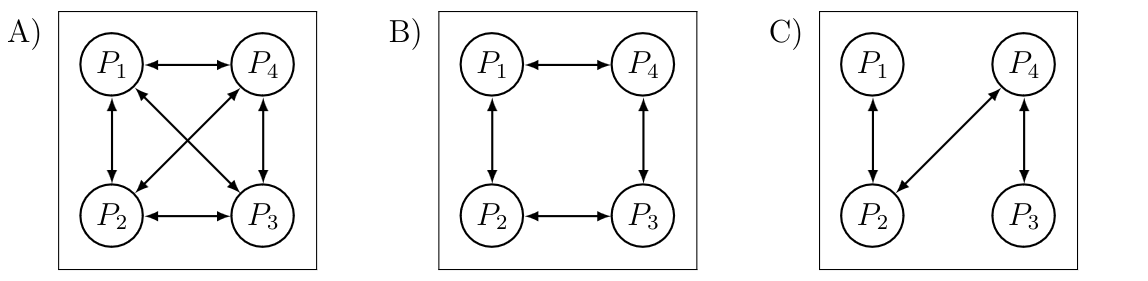
\includegraphics[scale=0.35]{p2p.png}}\\
\\
Assume you are asked to design communication protocols for each of these systems, such that the following
specification is implemented:\\
\\
\texttt{A message} $m$ \texttt{sent by any process} $P_i$ \texttt{is delivered to all other processes}
$P_j, j \neq i$\texttt{, exactly once and all at the same time.}\\
\\
A colleague of yours proposes the following protocol for System A (fully interconnected):\\
\\
A) sender protocol:
\begin{lstlisting}[style=CStyle]
t <- clock.now();
send (m, t) to neighbours;
\end{lstlisting}
A) receiver protocol:
\begin{lstlisting}[style=CStyle]
(m, t) <- receive();
delayUnit(t + d);
deliver(m);
\end{lstlisting}
a) With the described system model, is it possible to modify the proposed protocol such that it meets the
specification? Justify!\\
\\
The assumption must be made that all the processes $P_j$ for $i \neq j$ receive the messages before the
upper bound is hit. With the communication being synchronous that might not be the case, since all sends
and all receives are blocking. Since the loop on the sender side each iteration is waiting until the send 
call is executed and until the receive call was executed and the receiver send it's acknowledge to the 
sender. Under circumstances this overhead causes a huge enough delay that the upper delay already expired 
and since the sender is not checking if its sending messages while the delay is not expired it can not be 
sure that the messages are all delivered to the receiving processes at the same point of time. Further 
the receivers are acknowledging the received messages before evaluating if the contract to respect the 
delay can be met and errors only occur after the blocking of the receive call when the communication with 
$P_i$ has already happened. In conclusion I would suggest implementing a mechanism to check on the sender
side if the delay requirement can still be met:\\
\\
A) sender protocol:
\begin{lstlisting}[style=CStyle]
t <- clock.now() + d;
i <- 0;
for neighbours.length() < i {
  send (m, t) to neighbours[i];
  if t < clock.now() {
    error(wasn't able to deliver message in time);
  }
  i <- i + 1;
}
\end{lstlisting}
A) receiver protocol:
\begin{lstlisting}[style=CStyle]
(m, t) <- receive();
delayUnit(t);
deliver(m);
\end{lstlisting}
If no error was thrown the sender can now be sure that all receivers were able to get their message at
the same point in time.\\
\\
b) What additional assumptions must be added to the system model (interaction and failure model) such
that the proposed protocol meets the specification?\\
\\
As stated in a) the proposed protocol doesn't account for the fact that receivers might receive messages
at the point of time that is already bigger than the point of time describing the delay. So in order for
the proposed protocol to work the assumption must be made that for all receivers the delay is not hit
before the receive call exits it's blocking state.\\
\\
For the remainder of this question, the additional assumptions that you derived in part b) are added to
the system model!\\
\\
c) With your new system model, design a similar procol fullfilling the given specification for System B
with minimal communication and storage requirements!\\
\\
B) sender protocol:
\begin{lstlisting}[style=CStyle]
t <- clock.now() + d;
for v in neighbours {
  // this.index is the index of this process
  send (m, t, this.index) to neighbours[i];
  if t < clock.now() {
    error(wasn't able to deliver message in time);
  }
}
\end{lstlisting}
B) receiver protocol:
\begin{lstlisting}[style=CStyle]
// index is the index sent by the sender
(m, t, index) <- receive();
for v in neighbours {
  if index < 0 {
    continue
  }
  if index == v.index {
    continue
  }
  if v.index != this.index + 1 and v.index != this.index - 3{
    continue
  }
  send (m, t, -1) to v;
}
delayUnit(t);
deliver(m);
\end{lstlisting}
This implementation works under the assumption that we only forward the message to one more process after
the initial round of sending. The original sender sends his index with the send so that the receiving
processes don't forward the message to the sender. Also the processes only forward the message to 
processes with an index of their index incremented by one or their index minus three (catching the case
that $P_1$ is the process needing the message to be forwarded). This ensures that the receiving processes 
don't forward the message both. Also the process receiving the forwarded message knows that it should not
further forward because the index -1 is sent when a message gets forwarded. That way it is ensured that
a message gets only forwarded one "round".\\
\\
d) With your new system model, design a similar protocol fullfilling the given specification for System
C with minimal communication and storage requirements!\\
\\
C) sender protocol:
\begin{lstlisting}[style=CStyle]
t <- clock.now() + d;
for v in neighbours {
  // this.index is the index of this process
  send (m, t, this.index) to neighbours[i];
  if t < clock.now() {
    error(wasn't able to deliver message in time);
  }
}
\end{lstlisting}
C) receiver protocol:
\begin{lstlisting}[style=CStyle]
// index is the index sent by the sender
(m, t, index) <- receive();
for v in neighbours {
  if index == v.index {
    continue
  }
  send (m, t, this.index) to v;
}
delayUnit(t);
deliver(m);
\end{lstlisting}
This time we don't have to cover the case that multiple processes might be trying to forward a message to
the same process. Thats why it is enough to limit a receiver to not be allowed to forward the message it 
received to the process it received it from.\\
\\
\subsection*{2. Three-Army-Problem}
In the following we discuss a variation of the Two-Army-Problem presented in the lecture. Similar to the
Two-Army-Problem, the goal of the Three-Army-Problem is to reach agreement among three divisions about
the order time of the attack. In this case, it must be guranteed that the largest division attack last.\\
\\
The protocol must be clearly devided into two phases:\\
\\
1. The divisions coordinate the \textbf{order of attack} (by division size)\\
\\
2. The largest division determines the \textbf{time of attack} and informs the other divisions.\\
\\
Furthermore, attacks of subsequent divisions should take place \textbf{at least 1 minute apart}.\\
Assume a synchronous system, where no errors occur on the communication channel. A messenger between any
two divisions may take up to $d$ minutes. You may assume that all divisions are of different size. An
arbitrary division initiates the protocol at time $t_0$.\\
Note: There is no drift between the division's clocks.\\
\\
a) Here, assume that the clocks of all three divisions are perfectly synchronized (i. e. no drift, no
clock skew). Briefly describe a protocol for the Three-Army-Problem that fulfils the following two
conditions:\\
\\
1. The time between the first attack and the last attack must be minimal.\\
2. The first attack should start as soon as possible (without violating the first condition).\\
\\
Illustrate your protocol through a time-space-diagram.\\
Provide the worst-case attack times (i. e. messenger time = $d$) for each division.\\
\\
\noindent\makebox[\textwidth]{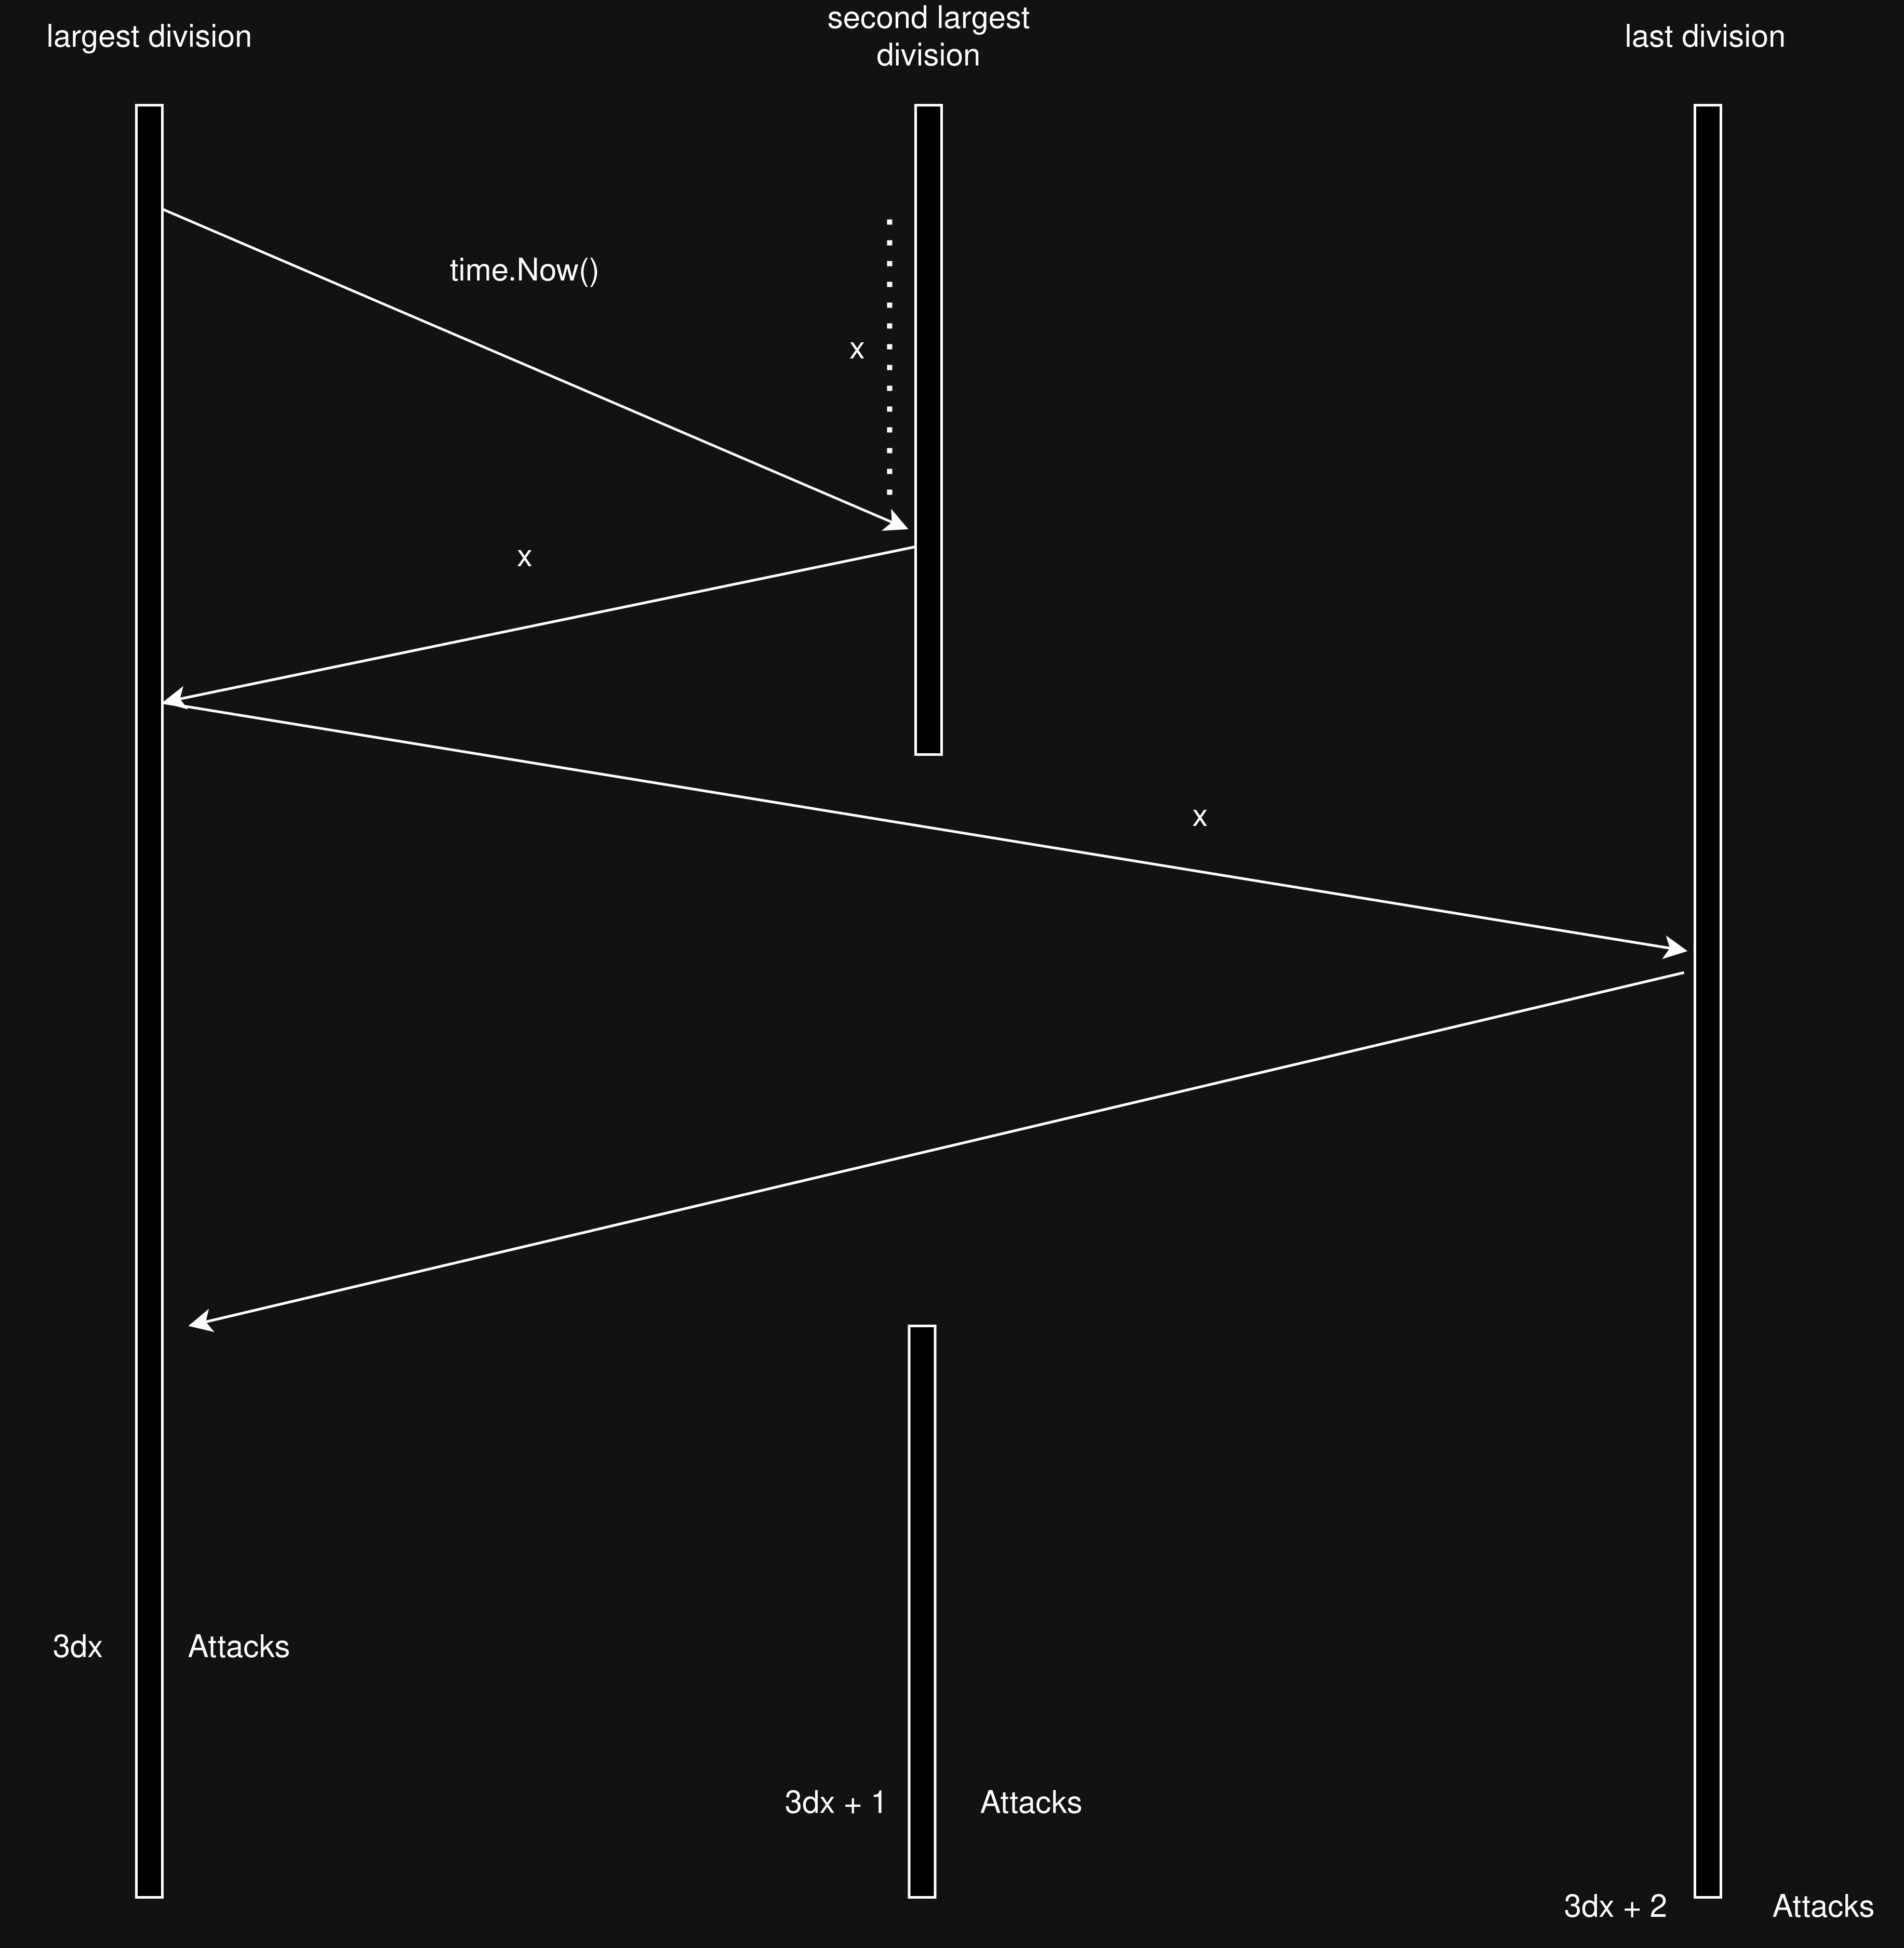
\includegraphics[scale=0.075]{clock.png}}\\
The first division sends the messenger to the second division and sends it's time stamp as the message.
Then the second division sends the messenger back for the acknowledge with the time stamp when they 
received the message. Then the messenger is send to the third devision with the message of the how long 
it took the messenger to deliver the first message. With that information exchange we let the first 
division attack after the duration of it's first send which will be $\leq d$ we will call 
that vairable $x$ and $3d$ since the other two divisions can't know how long their acknowledges took and 
also the second division can't know how long it took to deliver the message to the third division. We let 
the second division attack one second after the first division and the third two seconds after. In other 
words we let attack the first division at $3dx$ the second at $3dx + 1$ and the third $3dx + 2$ with $x$ 
being $\leq d$. In the worst case $x$ will be equal $d$ and therefore in the worst case the first 
division attacks at $4d$, the second at $4d + 1$ and the third at $4d + 2$. The only advantage we could 
take here was that we can measure how long the first send actually took and let all divisions know how 
long it took and eventually we don't have to wait one full delay.\\
\\
b) Now, assume that there may be an arbitrary clock skew (but no drift) between the clocks of different
divisions! Design a protocol that fulfils the two conditions given in part a), but with reversed priority,
that is:\\
\\
1. The first attack must start as soon as possible.\\
\\
2. The time between the first attack and the last attack should be minimal (without violating the first
condition).\\
\\
Again, briefly describe your protocol and illustrate it through a time-space-diagram and provide the
worst-case attack times (i. e. messenger time = $d$) for each division.\\
\\

\subsection*{3. Unreliable and Reliable Communication}

\end{document}
